 \documentclass[12pt, table]{article}
\usepackage[a4paper]{geometry}
%\newgeometry{left=2.2cm,bottom=2cm,right=2.2cm,top=2cm}
\usepackage{graphicx} % support the \includegraphics command and options
\usepackage{gensymb}
\usepackage{epsfig}
%\usepackage{graphicx}
\usepackage{caption}
\usepackage{subcaption}
%\usepackage{hyperref}
%%watermark{Draft}
\usepackage[printwatermark]{xwatermark}
\usepackage{lipsum}
\newwatermark[allpages,color=red!50,angle=45,scale=1.5,xpos=0,ypos=0]{DRAFT}
%%%[allpages,color=red!50,angle=45,scale=3,xpos=0,ypos=0]
\usepackage{amsmath}
%\usefonttheme{professionalfonts} 
\usepackage{float}
\usepackage{amsthm}
\usepackage{amssymb}
\usepackage{booktabs} % for much better looking tables
\usepackage{array} % for better arrays (eg matrices) in maths
\usepackage{paralist} % very flexible & customisable lists (eg. enumerate/itemize, etc.)
\usepackage{verbatim} % adds environment for commenting out blocks of text & for better verbatim
%\usepackage{subfig} % make it possible to include more than one captioned figure/table in a single
%\usepackage{booktabs}
\usepackage{tikz}
\usepackage{adjustbox}
\usepackage{natbib}
\bibliographystyle{agsm}
%\citestyle{aysep{char}}
\setcitestyle{aysep={},yysep={;}}
%\bibliographystyle{plain}
%%% HEADERS & FOOTERS
\usepackage{fancyhdr} % This should be set AFTER setting up the page geometry
\pagestyle{fancy} % options: empty , plain , fancy
\renewcommand{\headrulewidth}{0pt} % customise the layout...
\lhead{}\chead{}\rhead{}
\lfoot{}\cfoot{\thepage}\rfoot{}
\usepackage{sectsty}
\allsectionsfont{\sffamily\mdseries\upshape} % (See the fntguide.pdf for font help)
\usepackage{tabularx}
\usepackage[nottoc,notlof,notlot]{tocbibind} % Put the bibliography in the ToC
\usepackage[titles,subfigure]{tocloft} % Alter the style of the Table of Contents nm
\renewcommand{\cftsecfont}{\rmfamily\mdseries\upshape}
\renewcommand{\cftsecpagefont}{\rmfamily\mdseries\upshape} % No bold!
\newtheorem{conjecture}{Conjecture}
\newtheorem{lemma}{Lemma}
\newtheorem{theorem}{Theorem}
\newtheorem{corollary}{Corollary}
\newtheorem{remark}{Remark}
\newtheorem{Proposition}{Proposition}
\let\checkmark\undefined
\usepackage{dingbat}
\usepackage{tikz}
\usetikzlibrary{arrows}
\usetikzlibrary{arrows,shapes}
\usepackage{dsfont}    
\usepackage{dsfont} 
\usepackage{breqn}                                            %For the double bar R symbol for Real Numbers
\usepackage{amsbsy}                                            %To be able to bold greek letters
\usepackage{authblk}
%\usepackage{natbib}
%\usepackage[table]{xcolor}
\definecolor{lightgray}{gray}{0.9}
\title{\textbf{ The approximate Bayesian computation algorithm for  size-structured population model  with application in estimating the parameters of population dynamics in a patchy environment} 
}
\author[1]{XX}
\author[1]{YY}
\author[1]{ZZ}
\affil[1]{Department of Ecology, Evolution, and Natural Resources, Rutgers University }
\usepackage{hyperref}
\usepackage{color}
\usepackage{colortbl}
\renewcommand{\theequation}{\thesection.\arabic{equation}}
\def\qed{\mbox{}\hfill\raisebox{-2pt}{\rule{5.6pt}{8pt}\rule{4pt}{0pt}}\medskip\par}
\def\vn{\vspace{3ex}\noindent}
\newcommand{\al}{\alpha}
\newcommand{\bt}{\beta}
\newcommand{\ba}{\begin{array} }
\newcommand{\ea}{\end{array} }
\newcommand{\be}{\begin{equation} }
\newcommand{\ee}{\end{equation} }
\newcommand{\baa}{\begin{align} }
\newcommand{\eaa}{\end{align} }
\newcommand{\da}{\delta}
\newcommand{\kal}{\kappa}
\newcommand{\Da}{\Delta}
\newcommand{\la}{\lambda}
\newcommand{\f}{\displaystyle\frac}
\newcommand{\il}{\displaystyle\int}
\newcommand{\li}{\lim\limits}
\newcommand{\n}{\noindent}
\newcommand{\vp}{\varphi}
\newcommand{\va}{\vartheta}
\newcommand{\ga}{\gamma}
\newcommand{\ep}{\epsilon}
\newcommand{\cL}{{\mathscr{L}}}
\newcommand{\ma}{{\mathcal{A}}}
\newcommand{\mab}{{\tilde{\mathcal{A}}}}
\newcommand{\ra}{\rightarrow}
\newcommand{\Og}{\Omega}
\newcommand{\og}{\omega}
\newcommand{\op}{\oplus}
\newcommand{\s}{\sum\limits}
\newcommand{\p}{\bar{P}}
\newcommand{\pt}{\tilde{P}}
\newcommand{\qtt}{\tilde{Q}}
\newcommand{\q}{\bar{Q}}
\newcommand{\sg}{\sigma}
\newcommand{\Sg}{\Sigma}
\newcommand{\T}{{\mathbb{T}}}
\newcommand{\J}{{\mathbb{J}}}
\newcommand{\C}{{\mathbb{C}}}
\newcommand{\R}{{\mathbb{R}}}
\newcommand{\A}{{\mathbb{A}}}
\newcommand{\Z}{{\mathbb{Z}}}
\newcommand{\I}{{\mathbb{I}}}
\newcommand{\N}{{\mathbb{N}}}
\newcommand{\X}{{\mathds{X}}}
\newcommand{\B}{{\mathscr{B}}}
\newcommand{\W}{{\mathcal{W}}}
\newcommand{\F}{{\mathcal{F}}}
\newcommand{\pa}{\partial}
\newcommand{\pc}{\preccurlyeq}
\newcommand{\crd}{{\rm C}_{\rm rd}}
\newcommand{\cf}{{\rm C}}
\newcommand{\del}{^{\Delta}}
\newcommand{\tx}[1]{\quad\mbox{#1}\quad}
\newcommand{\ove}[1]{\overline{#1}}
\newcommand{\norm}[1]{\left\|#1\right\|}
\newcommand{\vecc}[2]{\begin{bmatrix}#1\\#2\end{bmatrix}}
\newcommand{\veccc}[2]{\begin{bmatrix}#1\\[.5cm]#2\end{bmatrix}}
\newcommand{\tu}[1]{\textup{#1}}
\newcommand{\td}{\tilde}
\newcommand{\ve}{\varepsilon}
\newcommand{\iy}{\infty}
\newcommand{\ta}{\theta}
\newcommand{\om}{\ominus}
\newcommand{\vt}{\vartriangleleft}
\newcommand{\tde}{\tilde{\delta}}
\newcommand{\tr}{\tilde{\rho}}
\newcommand{\tq}{\trianglelefteq}
\newcommand{\vect}[1]{\boldsymbol{#1}}
\DeclareMathOperator{\Id}{Id} \DeclareMathOperator{\sgn}{sgn}
\DeclareMathOperator{\diag}{diag}
%%%%
%%%
\begin{document}
\maketitle
\begin{abstract}
\end{abstract}
\section{Introduction}
%%%%%
%%%

[Motivation and Background information here]\\\\
In this study, we describe a regression approximate  bayesian computation (RABC) algorithm  for parameter estimation and inference in a size-structured  population model. The study builds on the previous work of \citep{beaumont2002approximate, beaumont2010approximate, bertorelle2010abc} by describing and demonstrating the efficacy of the  ABC methodology for parameter estimation and inference in a sized-structured population models. Our results suggest that the ABC framework is a promising framework for  parameter estimation of a size-structured model. 

\section{Approximate bayesian computation}
[Describe the ABC frameworks here]

\section{Illustration}
 Here we present three examples to illustrate the effectiveness of the RABC framework in estimating parameters of a size-structured population model.  The models we consider describe the dynamics of juvenile, young adults and adult fish in a patchy marine environment in which movement  between patches is allowed.  Temperature is assumed to vary between patches.  The first example allows only adult fish to migrate from one patch to another and assumes that reproduction is a function of temperature.  In the  second example, we assume that a fraction of the produced larvae in a patch, gets disperse to other patches and ignore any other dispersal that may occur.  The reproduction rate in each patch, is considered to be a function of the temperature in the patch.  The third example like the first one, assumes that  only adult fish are allow to migrate from one patch to another. Unlike the first  and second examples, it assumes that the juvenile growth rate is a function of temperature. In all the examples, everything, including parameters, is considered to be random.
 
\subsection{Example 1: }
{\bf Model formulation:}  We consider a fish  population  in two patches. Let $J_i(t)$, $A_i(t)$ and $\bar{A}_i(t)$ respectively represent the sub-populations of the juvenile, young adults and and adults  in patch $i$, $i = 1,~2$ at time t.  Furthermore, we suppose  that the temperature in patch $1$ and 2 are respectively $T_1(t)=T(t)$ and $T_2(t)=T(t)+\delta$ where $\delta \in \mathbb{R}$.  We assume  that  juvenile's population in each patch  can change as  a result of reproduction (by adult fish) and  growth (transitioning to young adult fish). We consider the rate of  reproduction to be a  parabolic function of temperature i.e. rate of reproduction $\alpha(T_i(t))=-w(T_i(t)-T_i^0)^2+\alpha_0$, $i=1,~2$ where the point $(T_i^0,~\alpha_0)$  is the vertex of the parabola and $w$ the width of the parabola. We assume  that juveniles and young adults have  constant growth rates:  $g_j$ and $g_a$ respectively.  The death rates of young adults ($m_a$) and adults   ($m_{\bar{a}}$) are assumed to be equal (i.e $m_a=m_{\bar{a}}$ ). A compartmental diagram for this dynamics  is illustrated in  Figure \eqref{fig1}. 

 \begin{figure}[H]
\tikzstyle{decision} =  [rectangle, draw, fill=red!20, 
    text width=7em, text centered, rounded corners, minimum height=4em]
\tikzstyle{block} = [rectangle, draw, fill=blue!20, 
    text width=7em, text centered, rounded corners, minimum height=4em]
\tikzstyle{line} = [draw, -latex']
\tikzstyle{cloud} = [draw, ellipse,fill=red!20, node distance=3cm,
    minimum height=2em]
    
\begin{tikzpicture}[node distance = 3cm, auto]
    % Place nodes
    \node [block] (juvenile) {Juvenile ($J_1$)};
    \node [block, right of=juvenile, node distance=4cm] (young) {Young Adults ($A_1$)};
    \node [block, right of =young, node distance=4cm] (adults) {Adults ($\bar{A}_1$)};   
   % \node [cloud, right of=bacteria, node distance=7cm] (phage) {Phage population(P)};
%    \node [block, left of=evaluate, node distance=3cm] (update) {update model};
%    \node [decision, below of=evaluate] (decide) {is best candidate better?};
%    \node [block, below of=decide, node distance=3cm] (stop) {stop};
    % Draw edges
    \node [decision, below of=juvenile, node distance=4cm] (juvenile2) {Juvenile ($J_2$)};
    \node [decision, right of=juvenile2, node distance=4cm] (young2) {Young Adults ($A_2$)};
    \node [decision, right of =young2, node distance=4cm] (adults2) {Adults ($\bar{A}_2$)};   

    \path [line] (juvenile) --node [midway] (gj) {$g_{j}$} (young);
    \path [line] (juvenile2) --node [midway] (gj2) {$g_{j}$} (young2);
     \path [line] (young) --node [midway] (ga) {$g_{a}$} (adults);
    \path [line] (young2) --node [midway] (ga2) {$g_{a}$} (adults2);
    
    \path [line] (adults) -- +(0,2) -| node [near start] {$\alpha(T_1)$} (juvenile);
     \path [line] (adults2) -- +(0,-2) -| node [near start] {$\alpha(T_2)$} (juvenile2);
   
     \path [line, dashed] (adults) -- node [midway]  {$d=1-f_s$ } (adults2);
      \path [line, dashed] (adults2)-- node [midway]  { }  (adults);
  
     \path [line] (adults.east) -- +(1.5,0) node [midway] {$m_a$};
     %\draw[black, thick, ->]  (adults2) --  (west);
     \path [line] (adults2.east) -- +(1.5,0) node [midway] {$m_a$};
    \path [line] (young) -- +(0,-1.5) node [midway] {$m_a$};
     \path [line] (young2.north) -- +(0,1) node [midway] {$m_a$};
\end{tikzpicture}
\caption{A compartmental diagram for  a size-structured fish dynamics model with juvenile recruitment a function of temperature and dispersal only in the adult compartments}
\label{fig1}
\end{figure}
The system of discrete equations describing the   two-patch model is given by: 
 \begin{align}
 J_1(t+1)&=  J_1(t)+\text{Poisson$\left(\alpha(T_1)\bar{A}_1(t)\right)$}-f_1(J_1)\nonumber\\  
 A_1(t+1)&=  A_1(t)+f_1(J_1)-f_2(A_1)-\text{Poisson$\left(m_aA_1(t)\right)$}\\  
 \bar{A}_1(t+1)&=  f_s\left[\bar{A}_1(t)+f_2(A_1)-f_3(\bar{A}_1)\right]\nonumber\\&+(1-f_s)\left[\bar{A}_2(t)+f_2(A_2)-f_3(\bar{A}_2)\right]\nonumber\\
 J_2(t+1)&=  J_2(t)+\text{Poisson$\left(\alpha(T_2)\bar{A}_2(t)\right)$}-f_1(J_2)\nonumber\\  
 A_2(t+1)&=  A_2(t)+f_1(J_2)-f_2(A_2)-\text{Poisson$\left(m_aA_2(t)\right)$}\nonumber\\  
 \bar{A}_2(t+1)&=  f_s\left[\bar{A}_2(t)+f_2(A_2)-f_3(\bar{A}_2)\right]\nonumber\\&+(1-f_s)\left[\bar{A}_1(t)+f_2(A_1)-f_3(\bar{A}_1)\right]\nonumber
\end{align}
where $f_1(J_i)=\text{Poisson$\left(g_jJ_i(t)\right)$}$,  $f_2(A_i)=\text{Poisson$\left(g_aA_i(t)\right)$}$,  and $f_3(\bar{A}_i)= \text{Poisson$\left(m_a\bar{A}_i(t)\right)$}$, $i=1,2.$
\subsubsection{Simulation}
We simulated 200000 data sets. 
\begin{figure}[H]

   \centering
   \begin{subfigure}[b]{0.45\textwidth}
       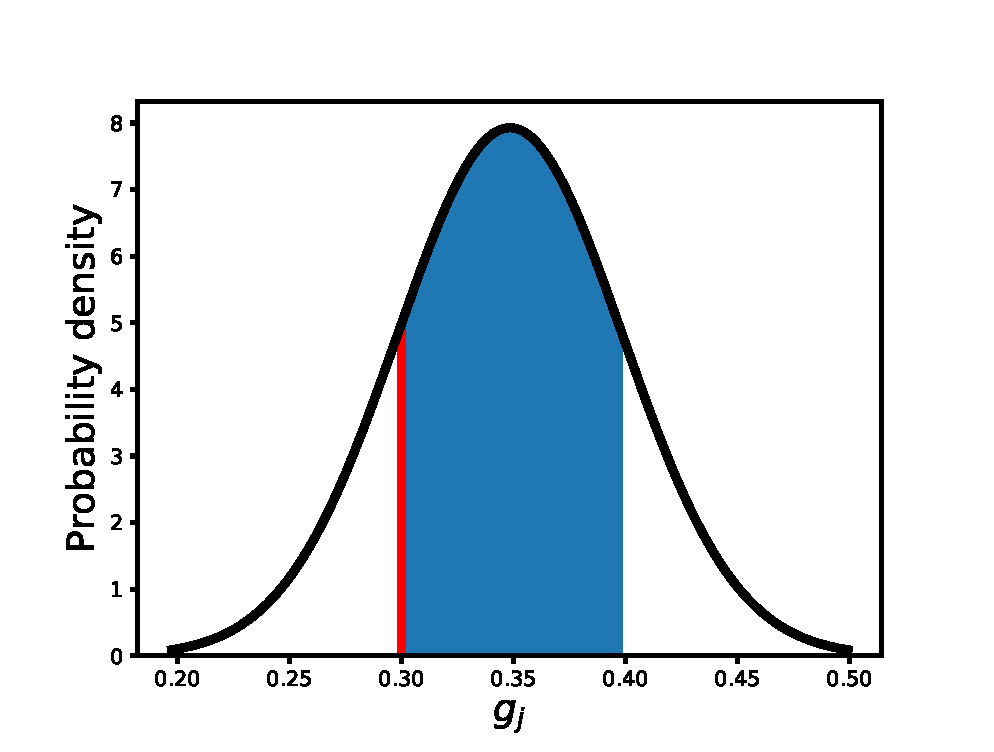
\includegraphics[width=1\textwidth, height=0.24\textheight]{figexple1/fgb}
      
       \caption{Growth rate of  juveniles.}
       % for  $N_{in}=0.02 mgCdm^{-3},~C_{in}=3mgCdm^{-3}$}
       \label{fig2a}
   \end{subfigure}
   ~ %add desired spacing between images, e. g. ~, \quad, \qquad, \hfill etc. 
     %(or a blank line to force the subfigure onto a new line)
   \begin{subfigure}[b]{0.45\textwidth}
       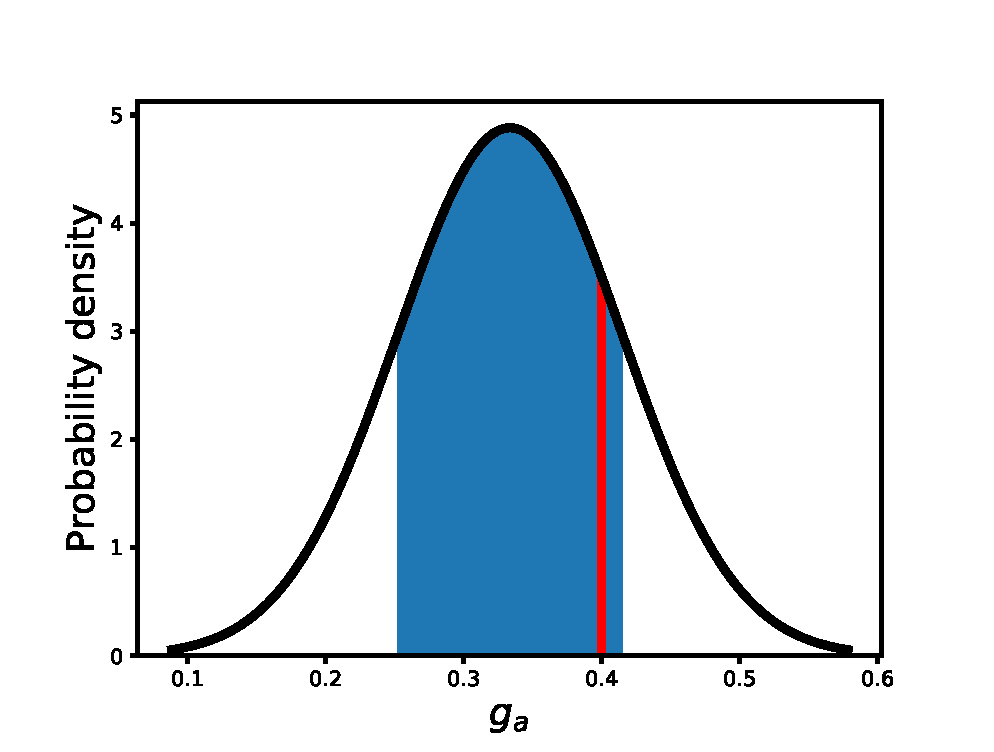
\includegraphics[width=1\textwidth, height=0.24\textheight]{figexple1/fgj}
        \caption{Growth rate of young adults.}
       \label{fig2b}
   \end{subfigure}\\
   \begin{subfigure}[b]{0.45\textwidth}
       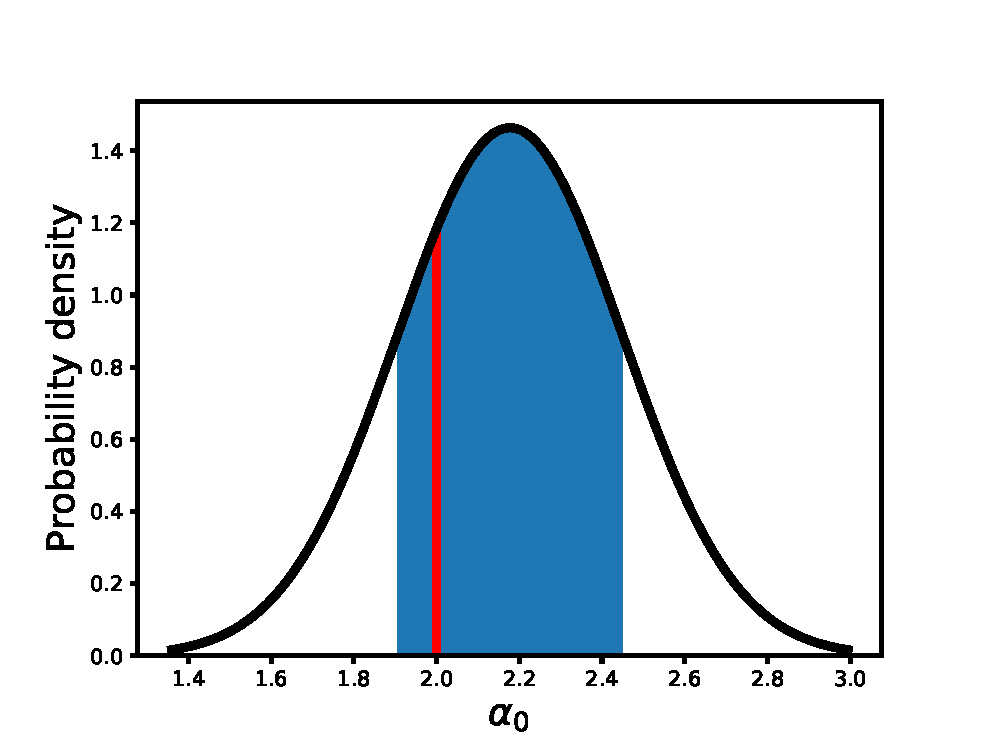
\includegraphics[width=1\textwidth, height=0.24\textheight]{figexple1/falpha0}
      
       \caption{Maximum reproduction  rate.}
       % for  $N_{in}=0.02 mgCdm^{-3},~C_{in}=3mgCdm^{-3}$}
       \label{fig2c}
   \end{subfigure}
   ~ %add desired spacing between images, e. g. ~, \quad, \qquad, \hfill etc. 
     %(or a blank line to force the subfigure onto a new line)
   \begin{subfigure}[b]{0.45\textwidth}
       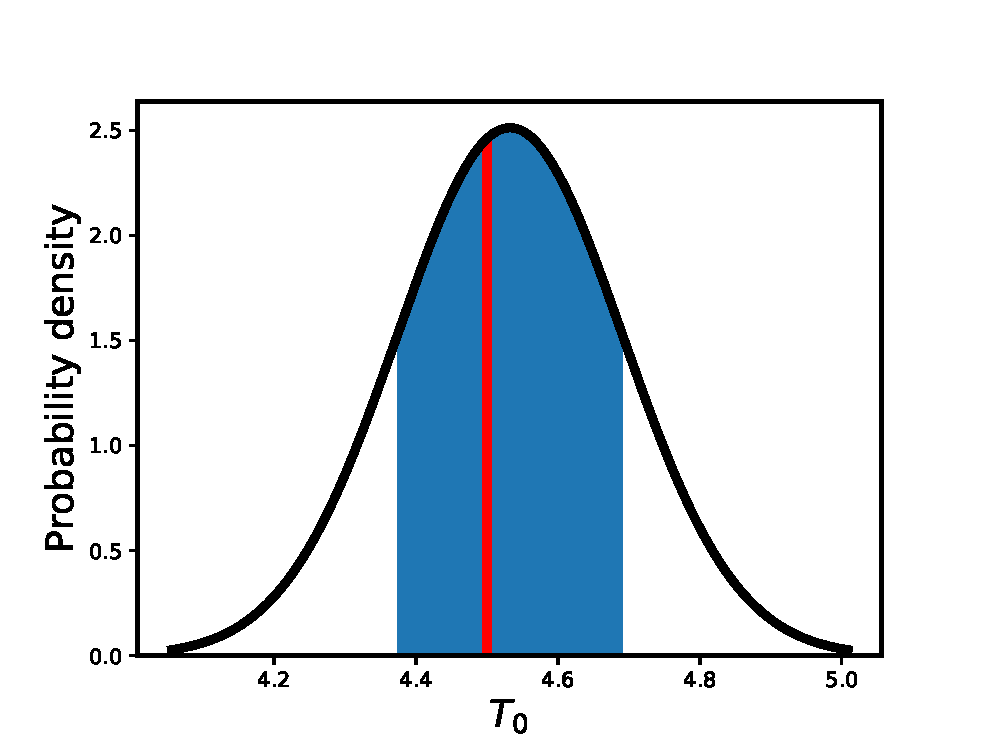
\includegraphics[width=1\textwidth, height=0.23\textheight]{figexple1/fT0}
        \caption{Temperature at maximum reproduction rate}
       \label{fig2d}
   \end{subfigure}\\
   \begin{subfigure}[b]{0.45\textwidth}
       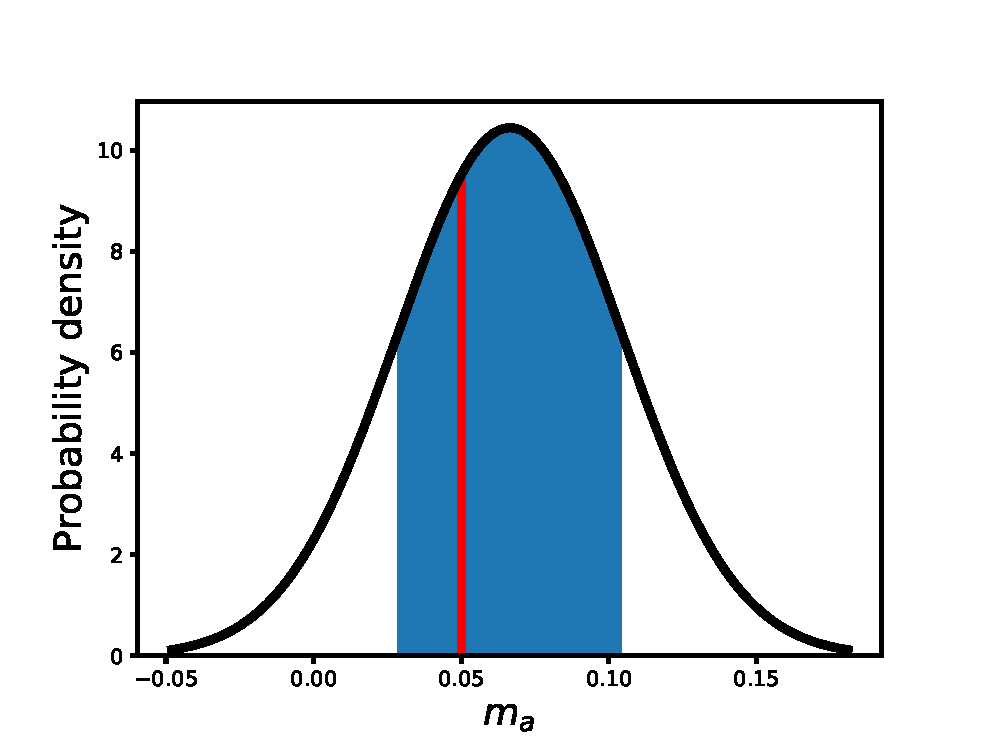
\includegraphics[width=1\textwidth, height=0.24\textheight]{figexple1/fmj}
        \caption{Death rate of  young adults.}
       \label{fig2e}
   \end{subfigure}
   \begin{subfigure}[b]{0.45\textwidth}
       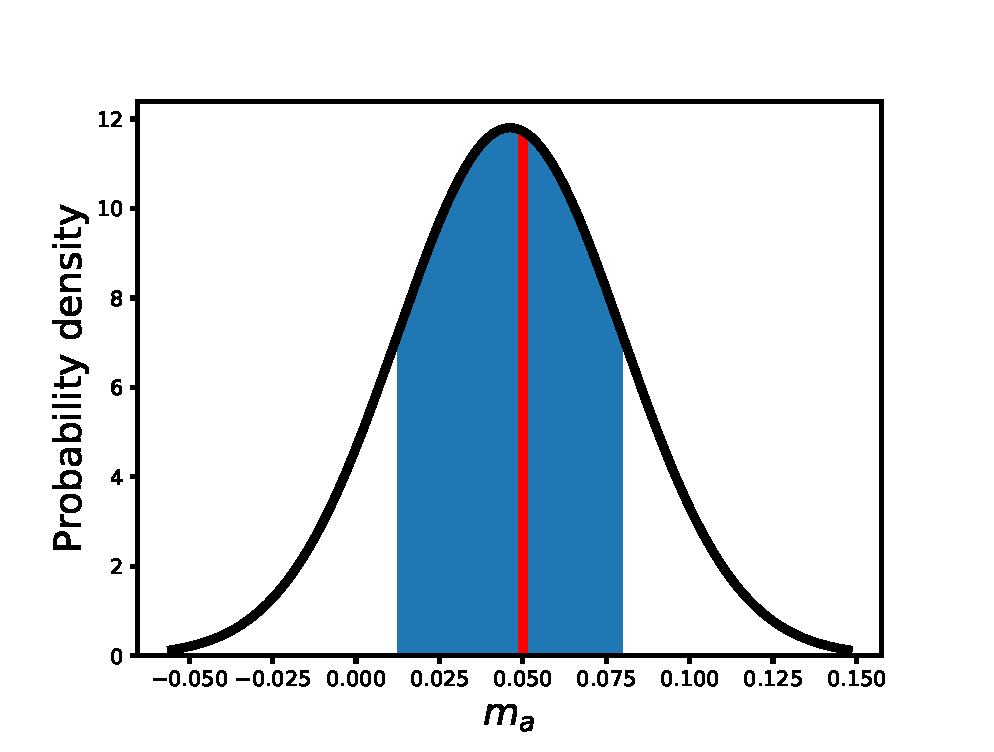
\includegraphics[width=1\textwidth, height=0.24\textheight]{figexple1/fma}
      
       \caption{Death rate of adults.}
       % for  $N_{in}=0.02 mgCdm^{-3},~C_{in}=3mgCdm^{-3}$}
       \label{fig2f}
   \end{subfigure}\\
   ~ %add desired spacing between images, e. g. ~, \quad, \qquad, \hfill etc. 
     %(or a blank line to force the subfigure onto a new line)
   \begin{subfigure}[b]{0.45\textwidth}
       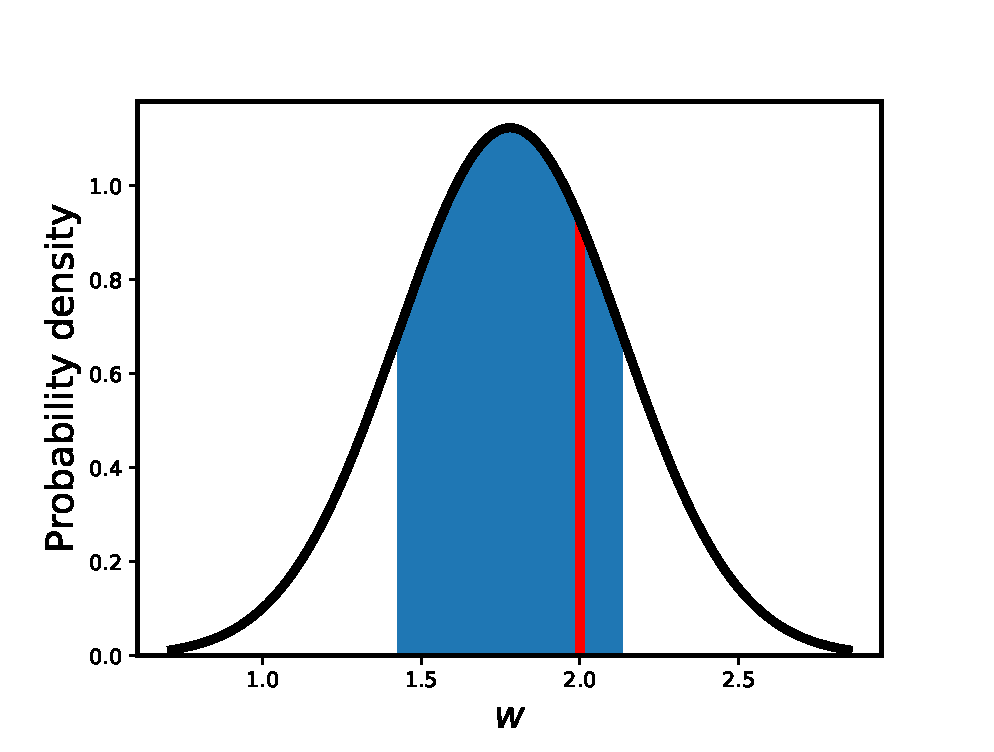
\includegraphics[width=1\textwidth, height=0.24\textheight]{figexple1/fwidth}
        \caption{width of parabola}
       \label{fig2g}
   \end{subfigure}
   ~ %add desired spacing between images, e. g. ~, \quad, \qquad, \hfill etc. 
     %(or a blank line to force the subfigure onto a new line)
   \begin{subfigure}[b]{0.45\textwidth}
       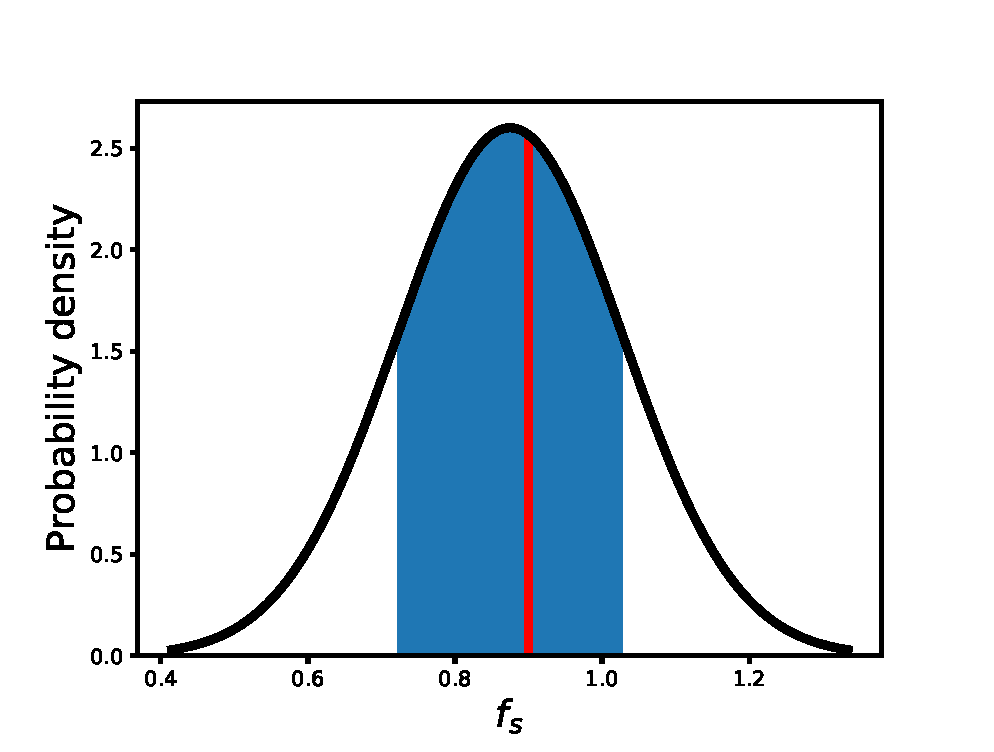
\includegraphics[width=1\textwidth, height=0.22\textheight]{figexple1/ffs}
        \caption{Fraction of adults  that remain in a compartment at each time}
       \label{fig2h}
   \end{subfigure}
\caption{Comparison of estimated vs observe values. Red line indicates the observed value, and the shaded section, the confidence interval of the estimated value}
   \label{fig2}
\end{figure}

\begin{table}[H]
\small
\begin{center}
 \rowcolors{1}{}{lightgray}
\begin{tabular}{lllll}
  \hline
  Parameter&Definition&True value&Estimated value& Confidence interval\\
  \hline
  $g_j$&-&0.3&0.3484&$(0.2980, 0.3987)$\\
  $g_a$&-&0.4&0.3335&$(0.2518, 0.4152)$\\
  $\alpha_0$&-&2&2.1774&(1.9048, 2.4499)\\
  $w$&-&2&1.7796&(1.4246, 2.1347)\\
  $f_s$&-&0.9&0.8747&$(0.7214,  1.0280)$\\
  $T_0$&-&4.5&4.5323&$(4.3735, 4.6911)$\\
  $m_a$&-&0.05&0.0665&$(0.0283   0.1047)$\\
  $m_a$&-&0.05&0.0461&$(0.0123,   0.0799)$\\
  \hline
\end{tabular}
\end{center}
\caption{Model parameter estimates}
\label{table1}
\end{table}

\subsection{Example 2:}
Example 2 captures a scenario in which only the  larvae are allowed to migrate from one patch to another.  We assume here that a fixed fraction $f_s$ of the produced larvae in a patch stays there and $1-f_s$ migrates   to another patch. The dynamics of the other compartments is  the same as those of the system  described in Example 1. 
%_=========================================
\begin{figure}[H]
\tikzstyle{decision} =  [rectangle, draw, fill=red!20, 
    text width=7em, text centered, rounded corners, minimum height=4em]
\tikzstyle{block} = [rectangle, draw, fill=blue!20, 
    text width=7em, text centered, rounded corners, minimum height=4em]
\tikzstyle{line} = [draw, -latex']
\tikzstyle{cloud} = [draw, ellipse,fill=red!20, node distance=3cm,
    minimum height=2em]
    
\begin{tikzpicture}[node distance = 3cm, auto]
    % Place nodes
    \node [block] (juvenile) {Juvenile ($J_1$)};
    \node [block, right of=juvenile, node distance=4cm] (young) {Young Adults ($A_1$)};
    \node [block, right of =young, node distance=4cm] (adults) {Adults ($\bar{A}_1$)};   
   % \node [cloud, right of=bacteria, node distance=7cm] (phage) {Phage population(P)};
%    \node [block, left of=evaluate, node distance=3cm] (update) {update model};
%    \node [decision, below of=evaluate] (decide) {is best candidate better?};
%    \node [block, below of=decide, node distance=3cm] (stop) {stop};
    % Draw edges
    \node [decision, below of=juvenile, node distance =6cm] (juvenile2) {Juvenile ($J_2$)};
    \node [decision, right of=juvenile2, node distance=4cm] (young2) {Young Adults ($A_2$)};
    \node [decision, right of =young2, node distance=4cm] (adults2) {Adults ($\bar{A}_2$)};   

    \path [line] (juvenile) --node [midway] (gj) {$g_{j}$} (young);
    \path [line] (juvenile2) --node [midway] (gj2) {$g_{j}$} (young2);
     \path [line] (young) --node [midway] (ga) {$g_{a}$} (adults);
    \path [line] (young2) --node [midway] (ga2) {$g_{a}$} (adults2);
    
    \path [line] (adults) -- +(0,2) -| node [near start] (al1){$f_s\alpha(T_1)$} (juvenile);
     \path [line] (al1) -- +(0,2) -| node [near start] {$(1-f_s)\alpha(T_1)$}(juvenile2.west);
     \path [line] (adults2) -- +(0,2) -| node [near start](al2) {$f_s\alpha(T_2)$} (juvenile2);
       \path [line] (al2) -- +(0,2) -|  node [near start] {$(1-f_s)\alpha(T_1)$}(juvenile.south);
%     \path [line, dashed] (adults) -- node [midway]  {$d=1-f_s$ } (adults2);
%      \path [line, dashed] (adults2)-- node [midway]  { }  (adults);
  
     \path [line] (adults.east) -- +(1.5,0) node [midway] {$m_a$};
     %\draw[black, thick, ->]  (adults2) --  (west);
     \path [line] (adults2.east) -- +(1.5,0) node [midway] {$m_a$};
    \path [line] (young) -- +(0,-1.5) node [midway] {$m_a$};
     \path [line] (young2.south) -- +(0,-1) node [midway] {$m_a$};
\end{tikzpicture}
\end{figure}

 \begin{align}
 J_1(t+1)&=  J_1(t)+f_sR(T_1(t), \bar{A}_1(t))+(1-f_s)R(T_2(t), \bar{A}_2(t))-f_1(J_1)\nonumber\\  
 A_1(t+1)&=  A_1(t)+f_1(J_1)-f_2(A_1)-\text{Poisson$\left(m_aA_1(t)\right)$}\\  
 \bar{A}_1(t+1)&=  \bar{A}_1(t)+f_2(A_1)-\text{Poisson$\left(m_a\bar{A}_1(t)\right)$}\nonumber\\
 J_2(t+1)&=  J_2(t)+(1-f_s)R(T_1(t), \bar{A}_1(t))+f_sR(T_2(t), \bar{A}_2(t))-f_1(J_2)\nonumber\\  
 A_2(t+1)&=  A_2(t)+f_1(J_2)-f_2(A_2)-\text{Poisson$\left(m_aA_2(t)\right)$}\nonumber\\  
 \bar{A}_2(t+1)&=  \bar{A}_2(t)+f_2(A_2)-\text{Poisson$\left(m_a\bar{A}_2(t)\right)$}\nonumber
\end{align}
where $f_1(J_i)=\text{Poisson$\left(g_jJ_i(t)\right)$}$ and  $f_2(A_i)=\text{Poisson$\left(g_aA_i(t)\right)$}$, $i=1,2.$


\begin{figure}[H]

   \centering
   \begin{subfigure}[b]{0.45\textwidth}
       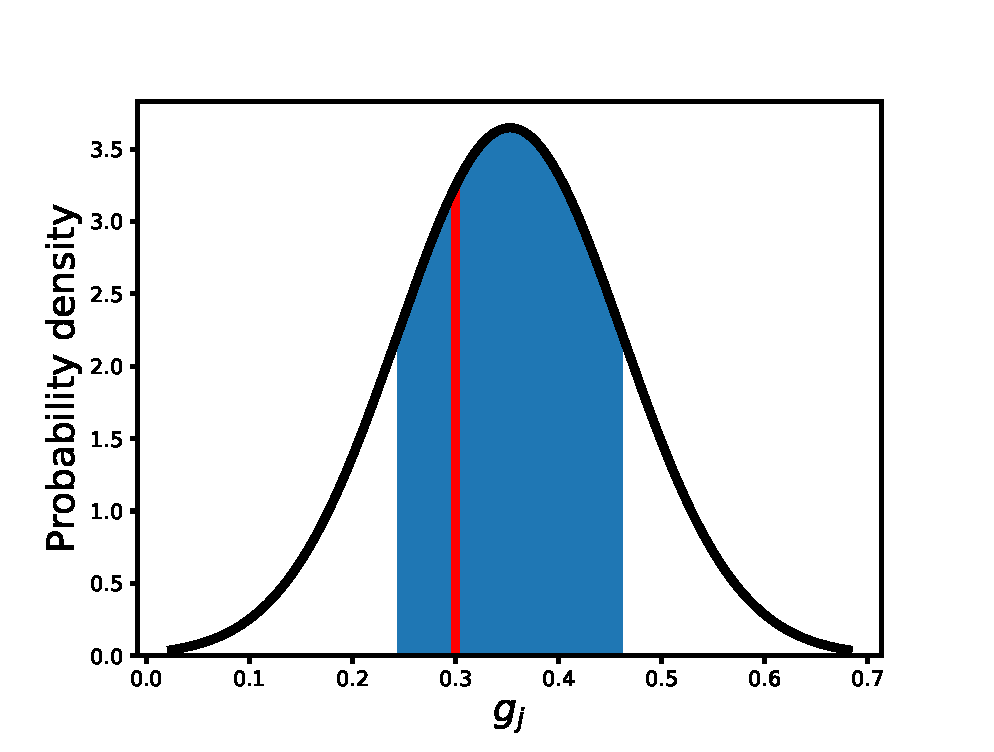
\includegraphics[width=1\textwidth, height=0.24\textheight]{figexple2/fgb}
      
       \caption{Growth rate of  juveniles.}
       % for  $N_{in}=0.02 mgCdm^{-3},~C_{in}=3mgCdm^{-3}$}
       \label{fig2a}
   \end{subfigure}
   ~ %add desired spacing between images, e. g. ~, \quad, \qquad, \hfill etc. 
     %(or a blank line to force the subfigure onto a new line)
   \begin{subfigure}[b]{0.45\textwidth}
       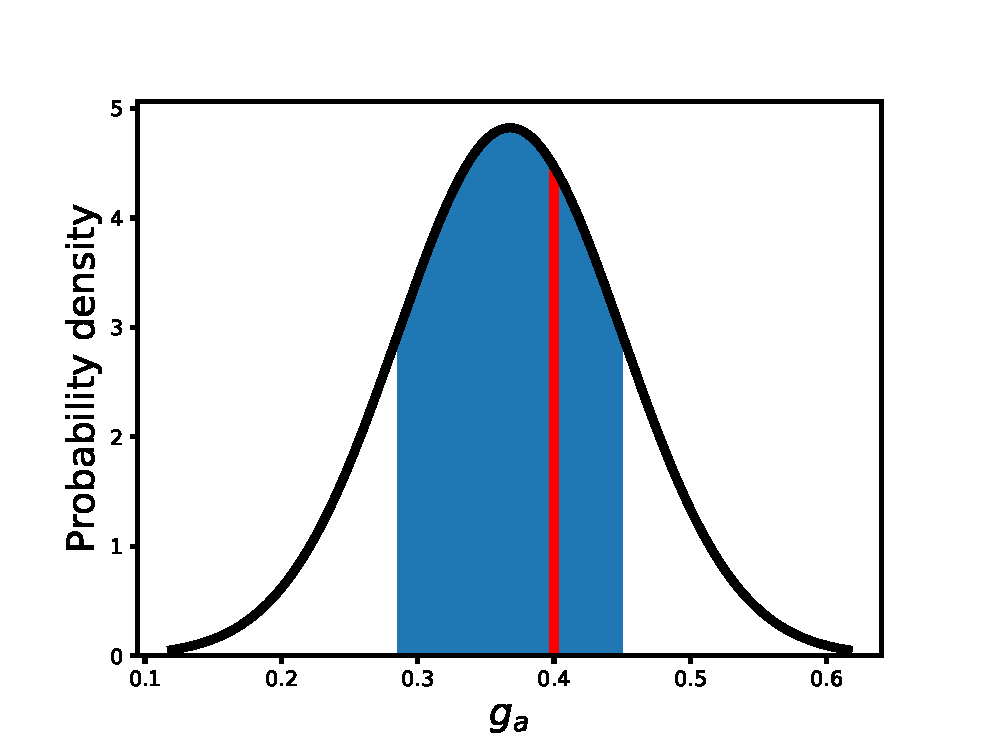
\includegraphics[width=1\textwidth, height=0.24\textheight]{figexple2/fgj}
        \caption{Growth rate of young adults.}
       \label{fig2b}
   \end{subfigure}\\
   \begin{subfigure}[b]{0.45\textwidth}
       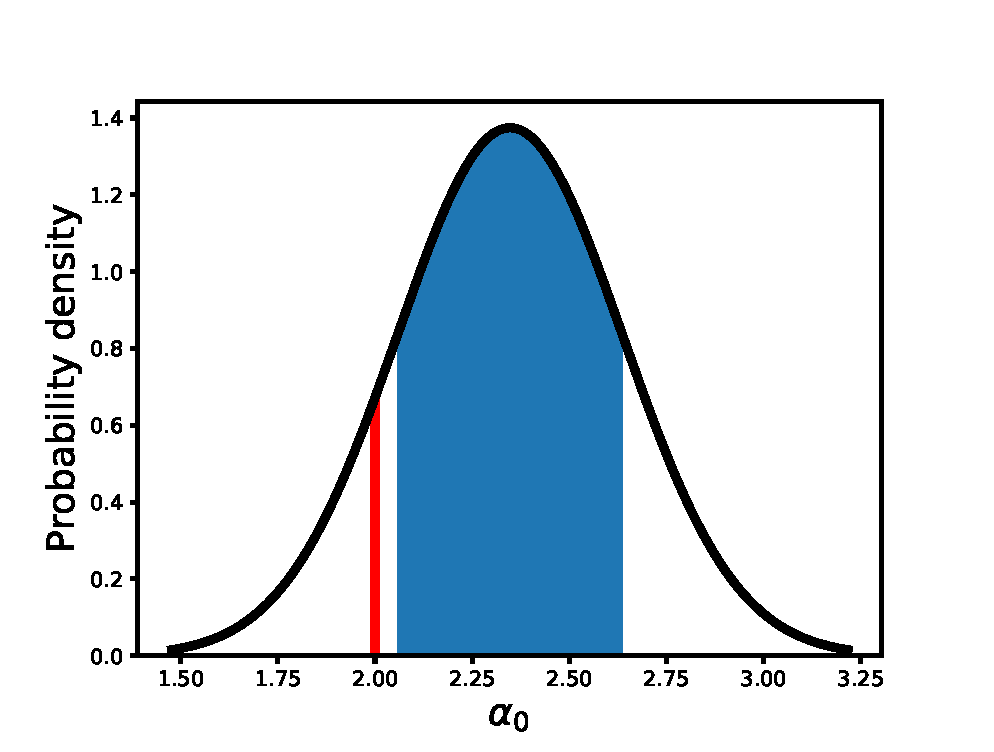
\includegraphics[width=1\textwidth, height=0.24\textheight]{figexple2/falpha0}
      
       \caption{Maximum reproduction  rate.}
       % for  $N_{in}=0.02 mgCdm^{-3},~C_{in}=3mgCdm^{-3}$}
       \label{fig2c}
   \end{subfigure}
   ~ %add desired spacing between images, e. g. ~, \quad, \qquad, \hfill etc. 
     %(or a blank line to force the subfigure onto a new line)
   \begin{subfigure}[b]{0.45\textwidth}
       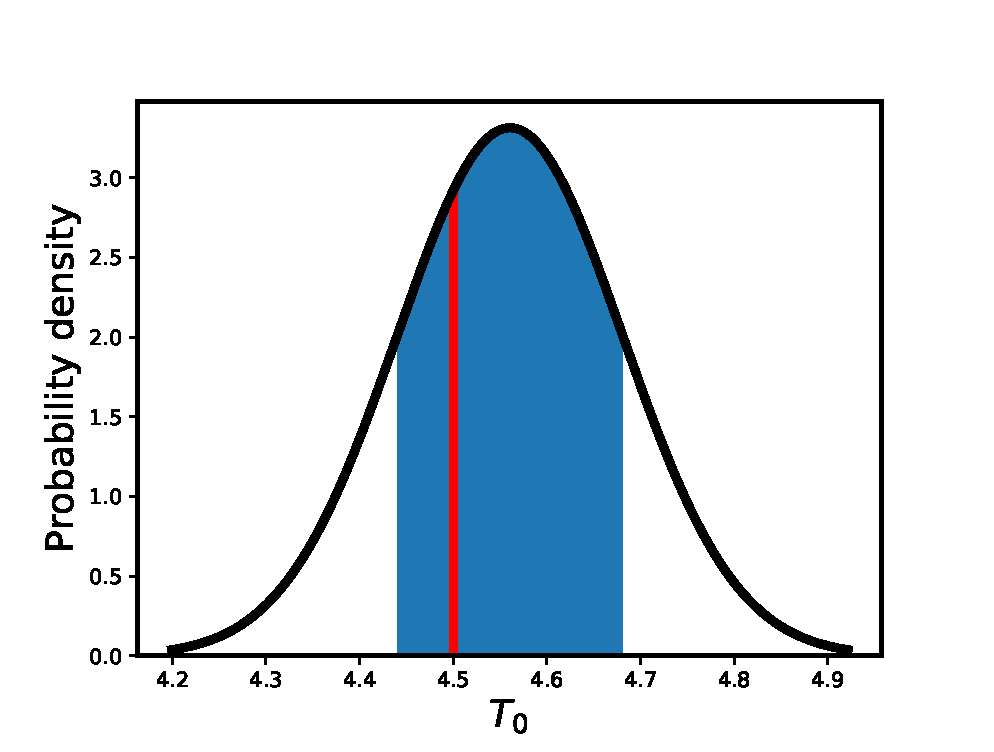
\includegraphics[width=1\textwidth, height=0.23\textheight]{figexple2/fT0}
        \caption{Temperature at maximum reproduction rate}
       \label{fig2d}
   \end{subfigure}\\
   \begin{subfigure}[b]{0.45\textwidth}
       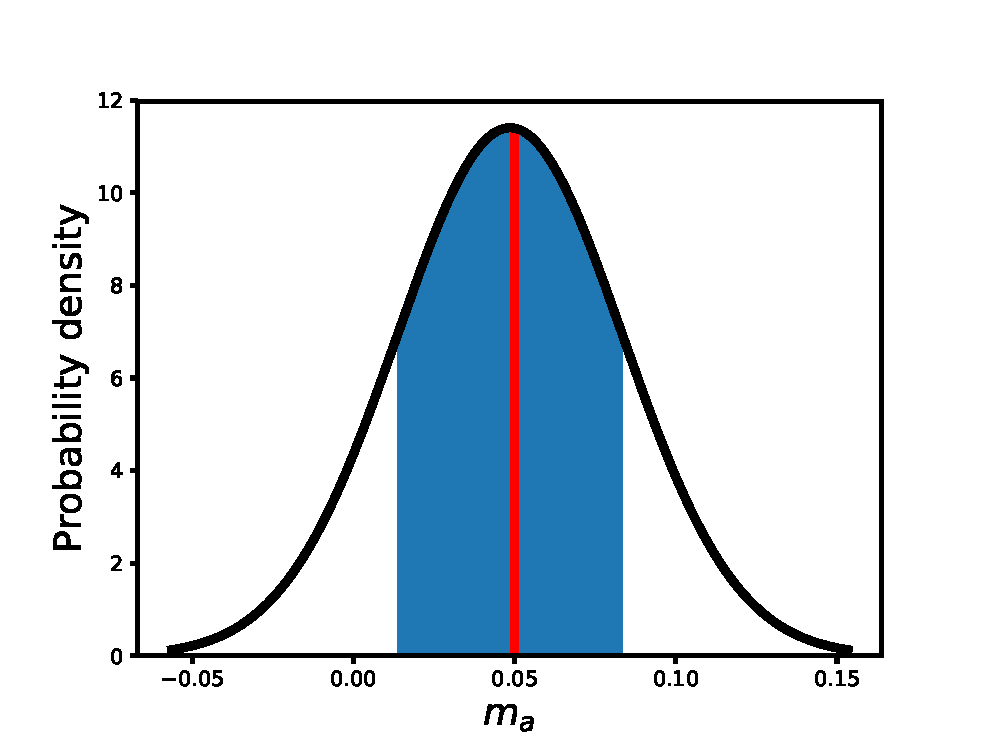
\includegraphics[width=1\textwidth, height=0.24\textheight]{figexple2/fmj}
        \caption{Death rate of  young adults.}
       \label{fig2e}
   \end{subfigure}
   \begin{subfigure}[b]{0.45\textwidth}
       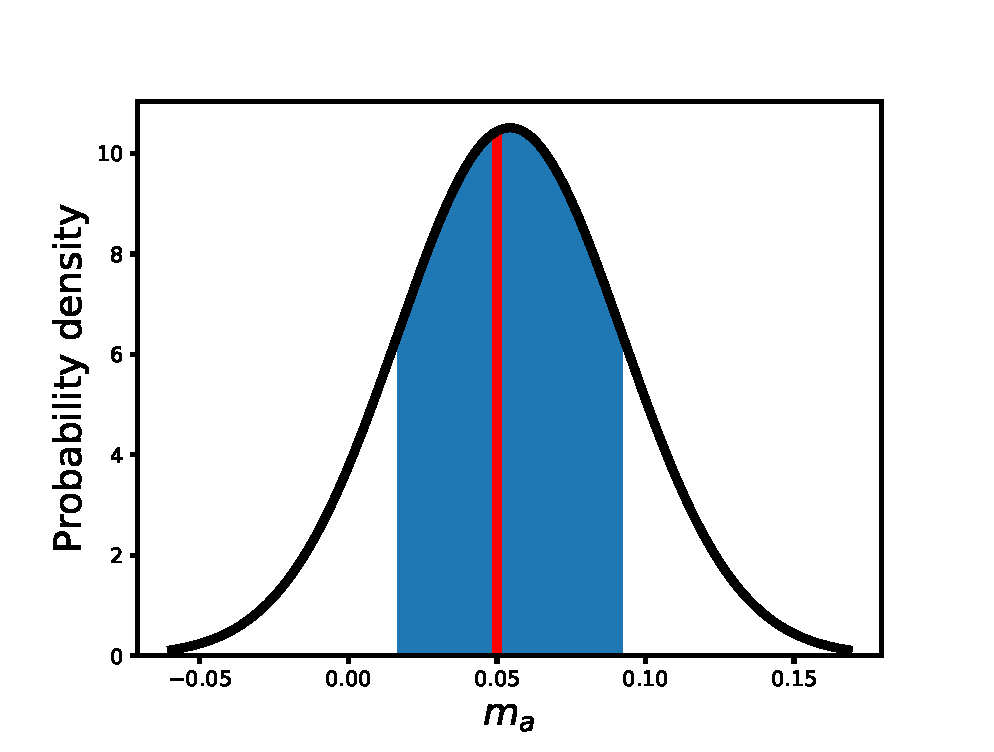
\includegraphics[width=1\textwidth, height=0.24\textheight]{figexple2/fma}
      
       \caption{Death rate of adults.}
       % for  $N_{in}=0.02 mgCdm^{-3},~C_{in}=3mgCdm^{-3}$}
       \label{fig2f}
   \end{subfigure}\\
   ~ %add desired spacing between images, e. g. ~, \quad, \qquad, \hfill etc. 
     %(or a blank line to force the subfigure onto a new line)
   \begin{subfigure}[b]{0.45\textwidth}
       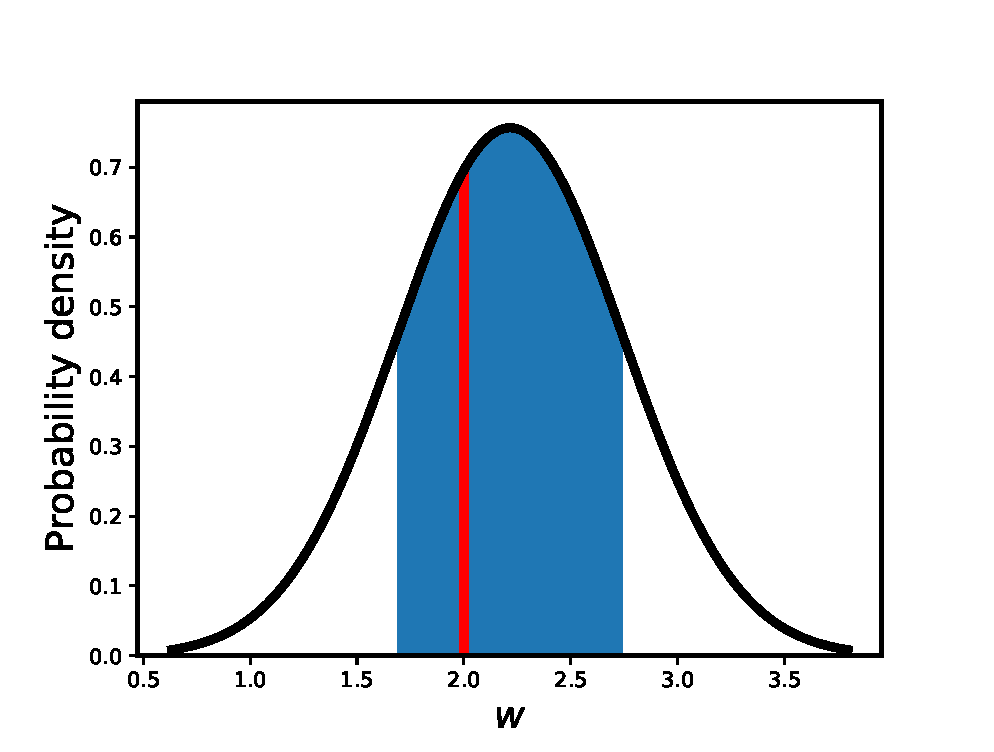
\includegraphics[width=1\textwidth, height=0.24\textheight]{figexple2/fwidth}
        \caption{width of parabola}
       \label{fig2g}
   \end{subfigure}
   ~ %add desired spacing between images, e. g. ~, \quad, \qquad, \hfill etc. 
     %(or a blank line to force the subfigure onto a new line)
   \begin{subfigure}[b]{0.45\textwidth}
       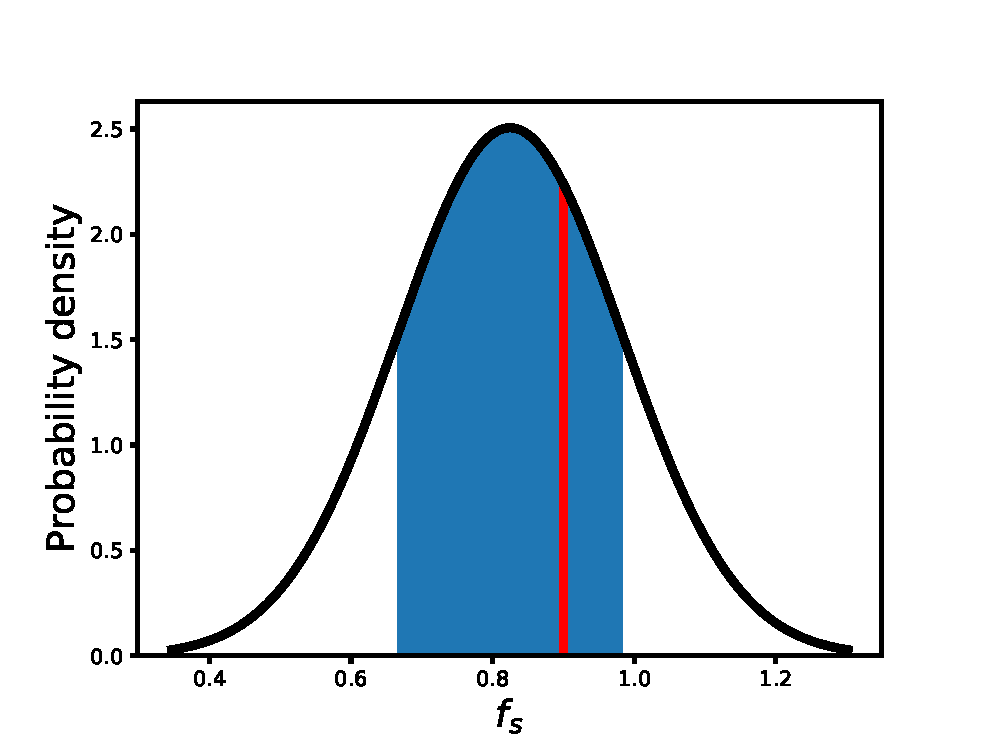
\includegraphics[width=1\textwidth, height=0.22\textheight]{figexple2/ffs}
        \caption{Fraction of adults  that remain in a compartment at each time}
       \label{fig2h}
   \end{subfigure}
\caption{Comparison of estimated vs observe values. Red line indicates the observed value, and the shaded section, the confidence interval of the estimated value}
   \label{fig2}
\end{figure}
  %_=========================================

\begin{table}[H]
\small
\begin{center}
 \rowcolors{1}{}{lightgray}
\begin{tabular}{lllll}
  \hline
  Parameter&Definition&True value&Estimated value& Confidence interval\\
  \hline
  $g_j$&-&0.3&0.3529&$( 0.24358, 0.4623)$\\
  $g_a$&-&0.4&0.3676&$(0.2849, 0.4503)$\\
  $\alpha_0$&-&2&2.3472&(2.0570,  2.6374)\\
  $w$&-&2&2.2151&(1.6878 2.7423)\\
  $f_s$&-&0.9&0.8244&$(0.6652, 0.9836)$\\
  $T_0$&-&4.5&4.5606&$(4.4402, 4.6810)$\\
  $m_a$&-&0.05&0.04855&$(0.0136, 0.0835)$\\
  $m_a$&-&0.05&0.0544&$(0.0164, 0.0923)$\\
  \hline
\end{tabular}
\end{center}
\caption{Model parameter estimates}
\label{table1}
\end{table}


\subsection{Example 3:}
Example 3 mimic a situation in which the reproduction rate is a constant $\alpha$ and the growth rate of juvenile to adult in each patch is a function of temperature $T_1(t)=T(t)$ and $T_2(t)=T(t)+\delta$ where $\delta \in \mathbb{R}$. The  temperature dependent growth rate is modelled using a parabolic function: $g_j(T_i(t))=-w(T_i(t)-T_i^0)^2+\alpha_0$, $i=1,~2$ where the point $(T_i^0,~\alpha_0)$  is the vertex of the parabola and $w$ the width of the parabola.  The dynamics of the other compartments is  the same as those of the system  described in Example 1. 
%For Example 1, we  consider a  two-patch  fish dynamic model.  Fish population in each patch is divided into three compartment: Juvenile, young adult fish and adult fish.  We denote the sizes of these groups by $J_i$, $A_i$ and $\bar{A}_i$ respectively  where $i=1,2.$ The recruitment  of juvenile fish is a function of temperature and temperature varies in the two patches. Migration between the two patches is only by matured adult fish. 

\begin{figure}[H]
\tikzstyle{decision} =  [rectangle, draw, fill=red!20, 
    text width=7em, text centered, rounded corners, minimum height=4em]
\tikzstyle{block} = [rectangle, draw, fill=blue!20, 
    text width=7em, text centered, rounded corners, minimum height=4em]
\tikzstyle{line} = [draw, -latex']
\tikzstyle{cloud} = [draw, ellipse,fill=red!20, node distance=3cm,
    minimum height=2em]
    
\begin{tikzpicture}[node distance = 3cm, auto]
    % Place nodes
    \node [block] (juvenile) {Juvenile ($J_1$)};
    \node [block, right of=juvenile, node distance=5cm] (young) {Young Adults ($A_1$)};
    \node [block, right of =young, node distance=4cm] (adults) {Adults ($\bar{A}_1$)};   
   % \node [cloud, right of=bacteria, node distance=7cm] (phage) {Phage population(P)};
%    \node [block, left of=evaluate, node distance=3cm] (update) {update model};
%    \node [decision, below of=evaluate] (decide) {is best candidate better?};
%    \node [block, below of=decide, node distance=3cm] (stop) {stop};
    % Draw edges
    \node [decision, below of=juvenile, node distance=4cm] (juvenile2) {Juvenile ($J_2$)};
    \node [decision, right of=juvenile2, node distance=5cm] (young2) {Young Adults ($A_2$)};
    \node [decision, right of =young2, node distance=4cm] (adults2) {Adults ($\bar{A}_2$)};   

    \path [line] (juvenile) --node [midway] (gj) {$g_{j}(T_1)$} (young);
    \path [line] (juvenile2) --node [midway] (gj2) {$g_{j}(T_2)$} (young2);
     \path [line] (young) --node [midway] (ga) {$g_{a}$} (adults);
    \path [line] (young2) --node [midway] (ga2) {$g_{a}$} (adults2);
    
    \path [line] (adults) -- +(0,2) -| node [near start] {$\alpha$} (juvenile);
     \path [line] (adults2) -- +(0,-2) -| node [near start] {$\alpha$} (juvenile2);
   
     \path [line, dashed] (adults) -- node [midway]  {$d=1-f_s$ } (adults2);
      \path [line, dashed] (adults2)-- node [midway]  { }  (adults);
  
     \path [line] (adults.east) -- +(1.5,0) node [midway] {$m_a$};
     %\draw[black, thick, ->]  (adults2) --  (west);
     \path [line] (adults2.east) -- +(1.5,0) node [midway] {$m_a$};
    \path [line] (young) -- +(0,-1.5) node [midway] {$m_a$};
     \path [line] (young2.north) -- +(0,1) node [midway] {$m_a$};
\end{tikzpicture}
\end{figure}
 \begin{align}
 J_1(t+1)&=  J_1(t)+\text{Poisson$\left(\alpha\bar{A}_1(t)\right)$}-f_1(J_1)\nonumber\\  
 A_1(t+1)&=  A_1(t)+f_1(J_1)-f_2(A_1)-\text{Poisson$\left(m_aA_1(t)\right)$}\\  
 \bar{A}_1(t+1)&=  f_s\left[\bar{A}_1(t)+f_2(A_1)-f_3(\bar{A}_1)\right]\nonumber\\&+(1-f_s)\left[\bar{A}_2(t)+f_2(A_2)-f_3(\bar{A}_2)\right]\nonumber\\
 J_2(t+1)&=  J_2(t)+\text{Poisson$\left(\alpha(T_2)\bar{A}_2(t)\right)$}-f_1(J_2)\nonumber\\  
 A_2(t+1)&=  A_2(t)+f_1(J_2)-f_2(A_2)-\text{Poisson$\left(m_aA_2(t)\right)$}\nonumber\\  
\bar{A}_2(t+1)&=  f_s\left[\bar{A}_2(t)+f_2(A_2)-f_3(\bar{A}_2)\right]\nonumber\\&+(1-f_s)\left[\bar{A}_1(t)+f_2(A_1)-f_3(\bar{A}_1)\right]\nonumber
\end{align}
where $f_1(J_i)=\text{Poisson$\left(g_jJ_i(t)\right)$}$,  $f_2(A_i)=\text{Poisson$\left(g_aA_i(t)\right)$}$,  and $f_3(\bar{A}_i)= \text{Poisson$\left(m_a\bar{A}_i(t)\right)$}$, $i=1,2.$

\begin{figure}[H]

   \centering
   \begin{subfigure}[b]{0.45\textwidth}
       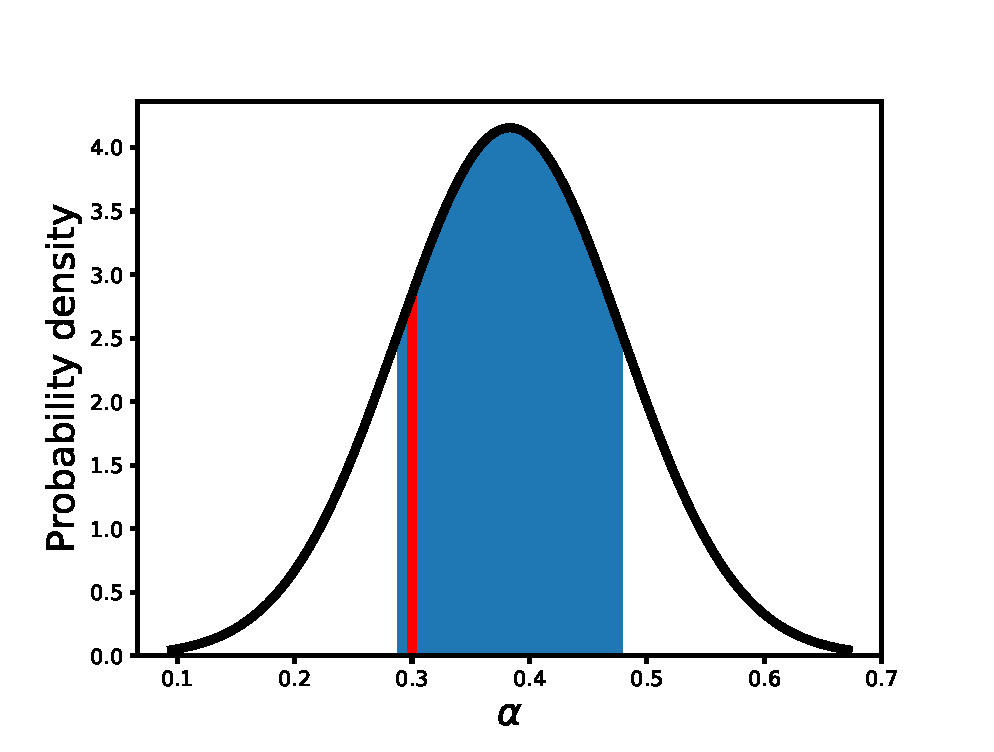
\includegraphics[width=1\textwidth, height=0.24\textheight]{figexple3/fgb}
      
       \caption{Growth rate of  juveniles.}
       % for  $N_{in}=0.02 mgCdm^{-3},~C_{in}=3mgCdm^{-3}$}
       \label{fig2a}
   \end{subfigure}
   ~ %add desired spacing between images, e. g. ~, \quad, \qquad, \hfill etc. 
     %(or a blank line to force the subfigure onto a new line)
   \begin{subfigure}[b]{0.45\textwidth}
       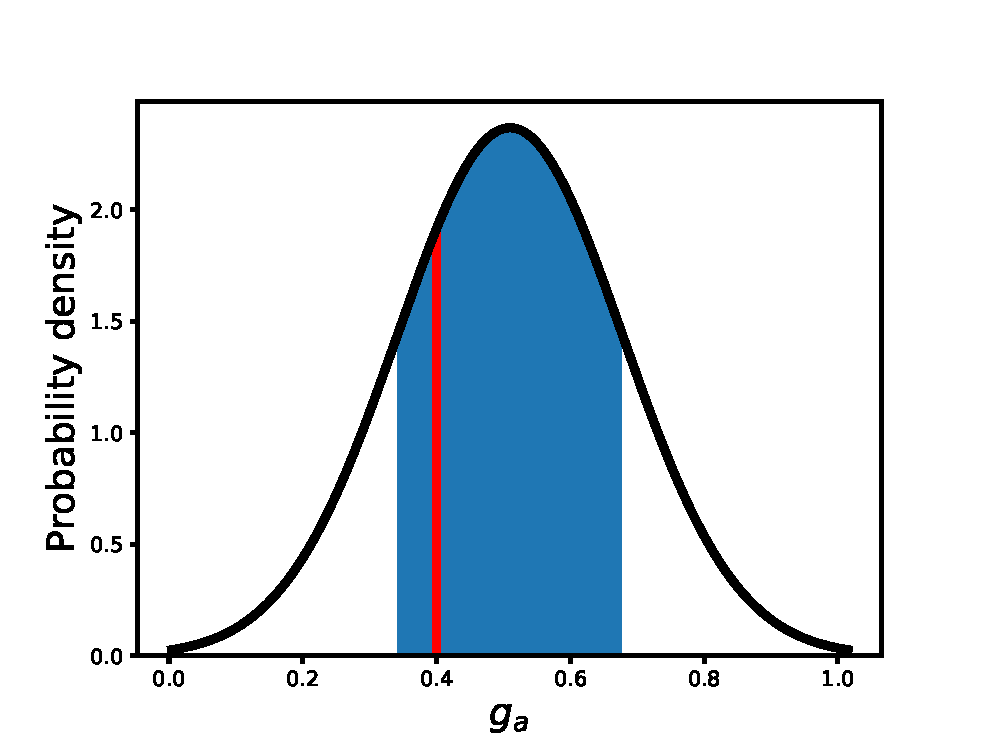
\includegraphics[width=1\textwidth, height=0.24\textheight]{figexple3/fgj}
        \caption{Growth rate of young adults.}
       \label{fig2b}
   \end{subfigure}\\
   \begin{subfigure}[b]{0.45\textwidth}
       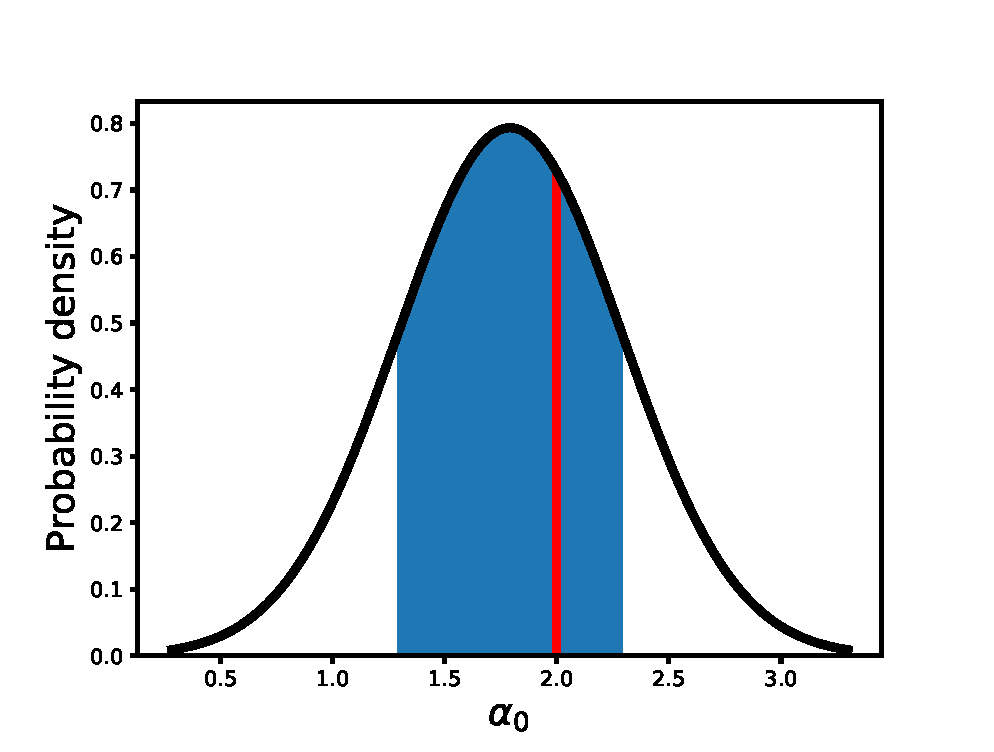
\includegraphics[width=1\textwidth, height=0.24\textheight]{figexple3/falpha0}
      
       \caption{Maximum reproduction  rate.}
       % for  $N_{in}=0.02 mgCdm^{-3},~C_{in}=3mgCdm^{-3}$}
       \label{fig2c}
   \end{subfigure}
   ~ %add desired spacing between images, e. g. ~, \quad, \qquad, \hfill etc. 
     %(or a blank line to force the subfigure onto a new line)
   \begin{subfigure}[b]{0.45\textwidth}
       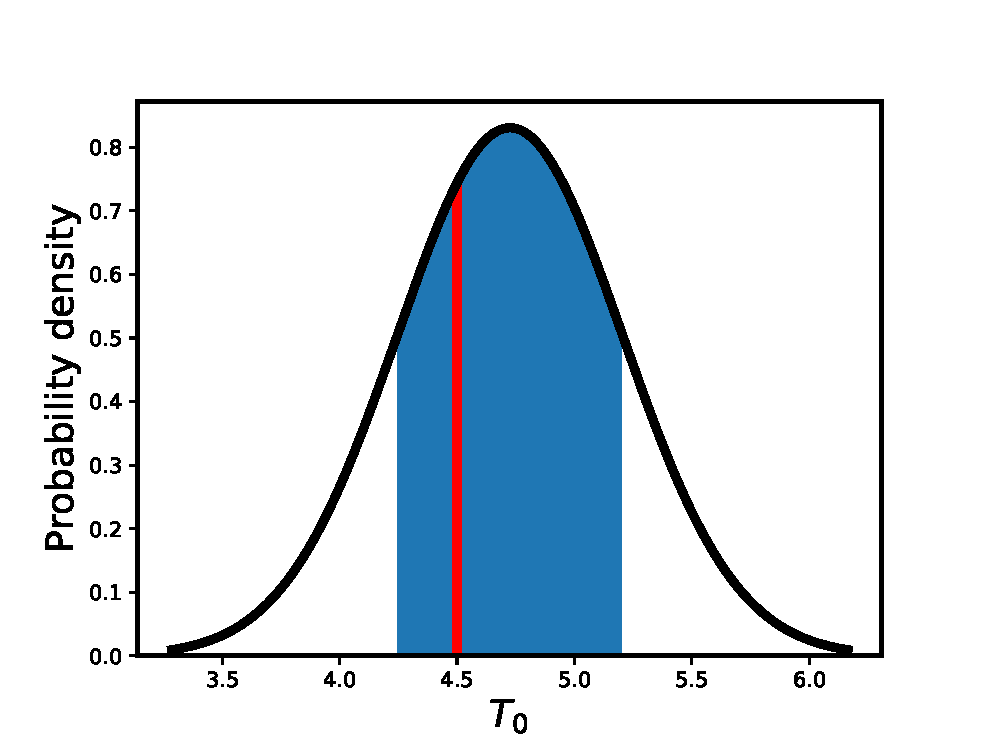
\includegraphics[width=1\textwidth, height=0.23\textheight]{figexple3/fT0}
        \caption{Temperature at maximum reproduction rate}
       \label{fig2d}
   \end{subfigure}\\
   \begin{subfigure}[b]{0.45\textwidth}
       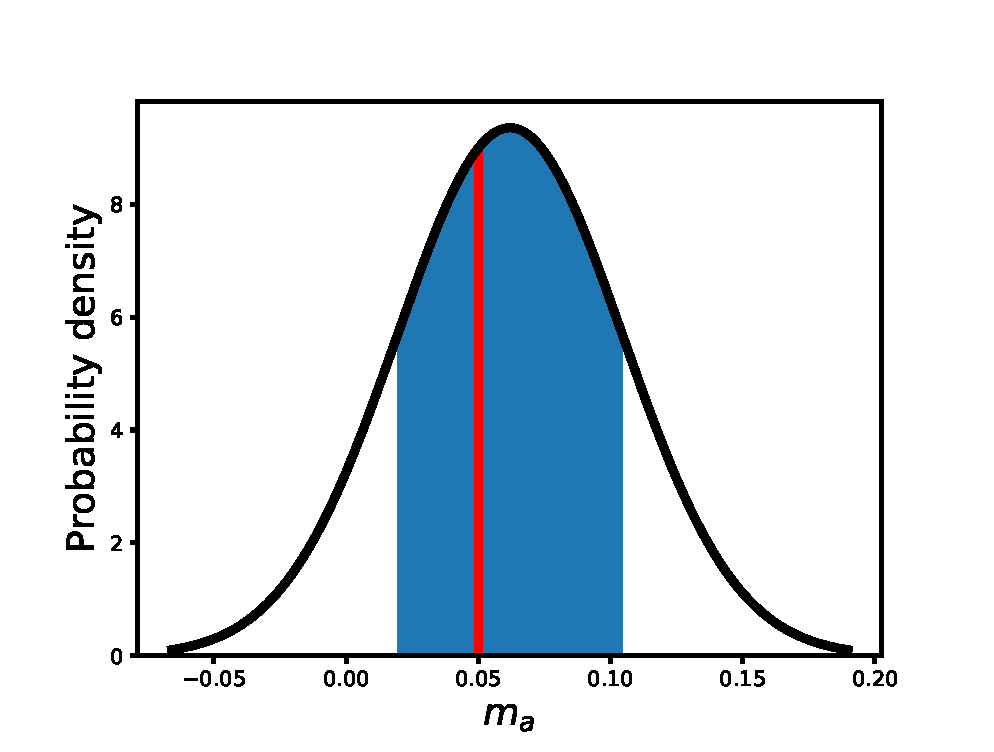
\includegraphics[width=1\textwidth, height=0.24\textheight]{figexple3/fmj}
        \caption{Death rate of  young adults.}
       \label{fig2e}
   \end{subfigure}
   \begin{subfigure}[b]{0.45\textwidth}
       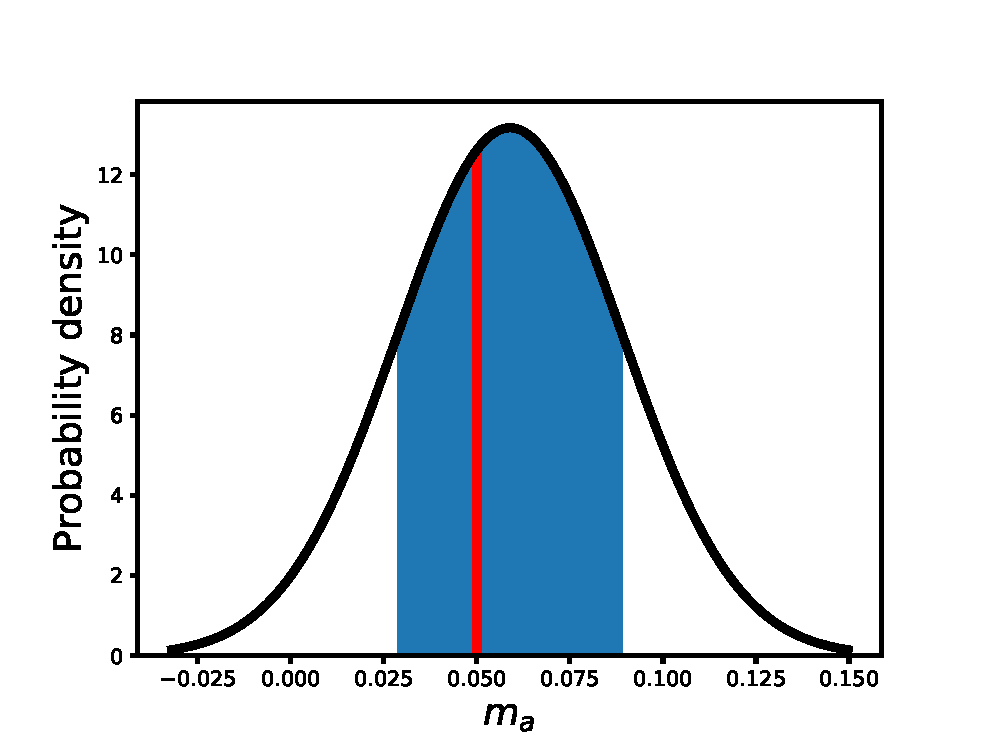
\includegraphics[width=1\textwidth, height=0.24\textheight]{figexple3/fma}
      
       \caption{Death rate of adults.}
       % for  $N_{in}=0.02 mgCdm^{-3},~C_{in}=3mgCdm^{-3}$}
       \label{fig2f}
   \end{subfigure}\\
   ~ %add desired spacing between images, e. g. ~, \quad, \qquad, \hfill etc. 
     %(or a blank line to force the subfigure onto a new line)
   \begin{subfigure}[b]{0.45\textwidth}
       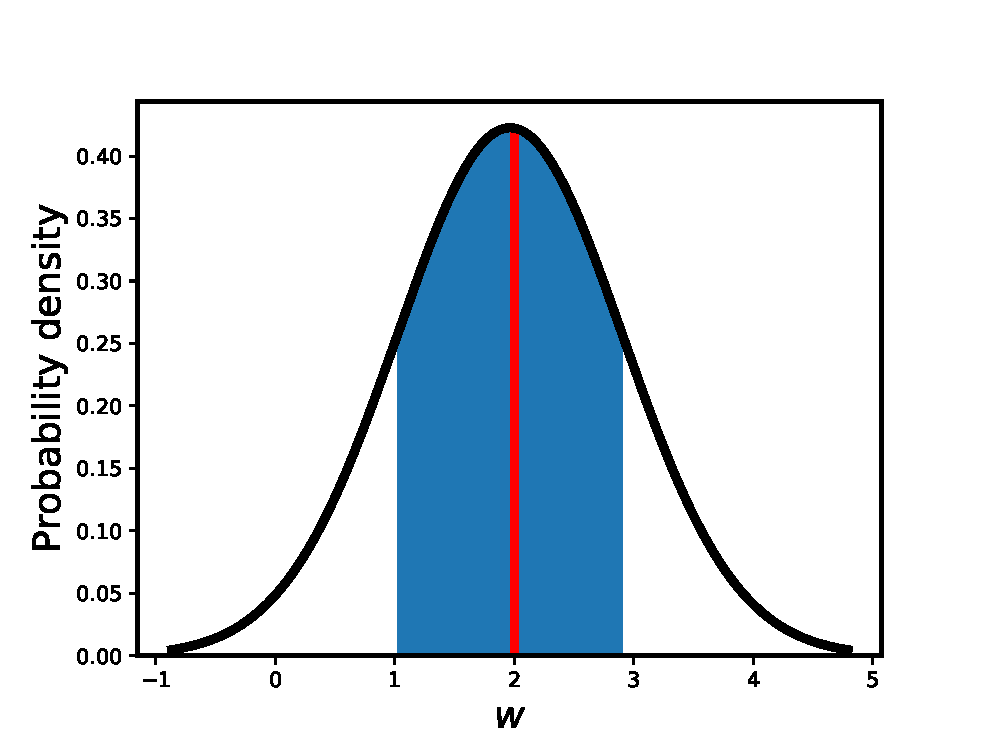
\includegraphics[width=1\textwidth, height=0.24\textheight]{figexple3/fwidth}
        \caption{width of parabola}
       \label{fig2g}
   \end{subfigure}
   ~ %add desired spacing between images, e. g. ~, \quad, \qquad, \hfill etc. 
     %(or a blank line to force the subfigure onto a new line)
   \begin{subfigure}[b]{0.45\textwidth}
       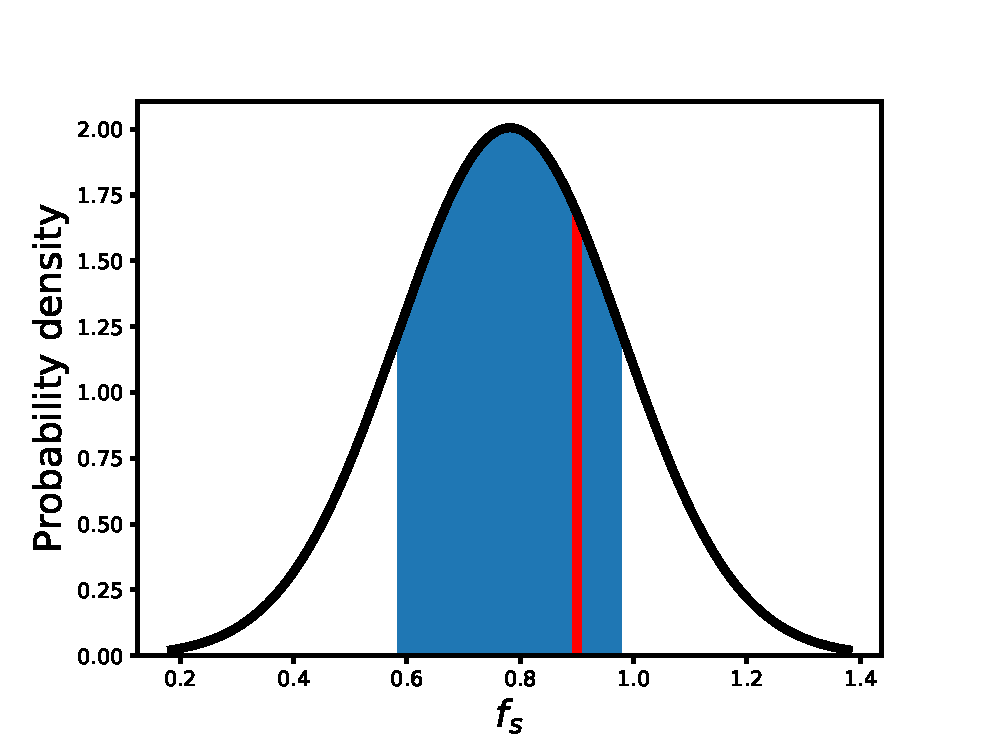
\includegraphics[width=1\textwidth, height=0.22\textheight]{figexple3/ffs}
        \caption{Fraction of adults  that remain in a compartment at each time}
       \label{fig2h}
   \end{subfigure}
\caption{Comparison of estimated vs observe values. Red line indicates the observed value, and the shaded section, the confidence interval of the estimated value}
   \label{fig2}
\end{figure}


\begin{table}[H]
\small
\begin{center}
 \rowcolors{1}{}{lightgray}
\begin{tabular}{lllll}
  \hline
  Parameter&Definition&True value&Estimated value& Confidence interval\\
  \hline
  $g_a$&-&0.4&0.5097&$(0.3412, 0.6782)$\\
  $\alpha$&-&0.3&0.3834&$(0.2874, 0.4793)$\\
  $\alpha_0$&-&2&1.7915&(1.2888, 2.2942)\\
  $w$&-&2&1.9633&(1.0196, 2.9070)\\
  $f_s$&-&0.9&0.7819&$(0.5830, 0.9808)$\\
  $T_0$&-&4.5&4.7252&$(4.2451, 5.2054)$\\
  $m_a$&-&0.05&0.0620&$(0.0193,  0.1046)$\\
  $m_a$&-&0.05&0.0589&$(0.0286 0.0892)$\\
  \hline
\end{tabular}
\end{center}
\caption{Model parameter estimates}
\label{table1}
\end{table}


\section{Conclusion}

 \bibliography{refs}
\end{document}
